\setlength{\marginparsep}{.5cm}
\setlength{\marginparwidth}{2cm}
%\addtolength{\marginparwidth}{2cm}


%#######################################################################
%################# on change les noms des tableaux et des figures
%#######################################################################
\addto\captionsfrench{\def\figurename{{Figure}}} 
\addto\captionsfrench{\def\tablename{{Tableau}}}


%#######################################################################
%################# définition de commandes supplémentaires
%#######################################################################


%#######################################################################
%################# Options de compilation
%#######################################################################

\def\ChoixDeVersion{PASprof} % soit {prof} et alors les commentaires profs sont ajoutés, soit autre chose

\newcommand{\prof}[1]{
        \ifthenelse{
                \equal{\ChoixDeVersion}{prof}
                }{\vspace{6pt}
                
                \vspace{12pt}\includegraphics[angle=0,width=1.5cm]{./images/prof} \textbf{Professeur :} \textsl{#1}
                
                \vspace{12pt}}{}
}

% remarque : pour compiler
% pdflatex --jobname=versionA '\def\ChoixDeVersion{prof}\input{source.tex}'      


%#######################################################################
%################# Définitions des boites prêtes à l'emploi...
%#######################################################################

% \usepackage{tikz} il est déjà chargé ici
\newcommand*\circled[1]{\tikz[baseline=(char.base)]{
            \node[shape=circle,draw,inner sep=1pt] (char) {#1};}}

% une boîte TODO
\newcommand{\todo}[1]{\vspace{12pt}


\includegraphics[angle=0,width=2cm]{./images/todo} \textbf{#1}
                
                \vspace{12pt}
}



% une boite : boite
\newcommand{\boite}[1]{%
\colorbox{rougeClair}{\parbox{\textwidth}{#1}}
}

% une boite : boite Enoncé
\newcommand{\boiteEnonce}[1]{%
\colorbox{couleurVinci}{\parbox{\textwidth}{\vspace{4pt}\textsl{#1}\vspace{4pt}}}
\vspace{8pt}
}

% la même version, mais avec un espace plus large au bord :
\newcommand{\boiteEnonceLarge}[1]{%
\colorbox{couleurVinci}{\parbox{\textwidth}{
\begin{center}\begin{minipage}[c]{.95\textwidth}
#1  
\end{minipage}\end{center}}}
\vspace{8pt}
}



% une boite encadrée : cadre À retenir
\newcommand{\cadre}[1]{% 
\vspace{12pt}
\parbox{\textwidth}{\textsl{\textbf{\textcolor{defaultColor}{À retenir...}}}\vspace*{4pt}\newline
\framebox{\parbox{\textwidth}{#1}}}
\vspace{12pt}
}

\newcommand{\cadreLarge}[1]{%
\framebox{\parbox{\textwidth}{
\begin{center}\begin{minipage}[c]{.95\textwidth}
#1  
\end{minipage}\end{center}}}
}



% une boite avec titre : boitetitre
\newlength{\textlarg}
\newcommand{\boitetitre}[2]{%
\settowidth{\textlarg}{\textbf{#1}}
\addtolength{\textlarg}{12pt}
\colorbox{ocre}{\parbox{\textwidth}{\hfill\rule[3pt]{.5\linewidth-.5\textlarg}{1pt}\hspace{5pt}\textbf{#1}\hspace{5pt}\rule[3pt]{.5\linewidth-.5\textlarg}{1pt}\hfill\phantom{.}\\[-12pt]#2}}}

% une boite dans la marge : boitemarge
\newcommand{\boitemarge}[1]{%
\marginpar{{\scriptsize #1

}}}


%
% une image ici
% 2 paramètres, 1:la taille, 2: l'échelle
\newcommand{\uneimageici}[2]{%
\vspace{8pt}
\begin{center}
\includegraphics[angle=0,width=#2]{#1}
\end{center}%
\vspace{8pt}
%\vspace{-18pt} % attention à ce vspace -18 qui peut créer des chevauchements
}%




%
% deux image ici
% 2 paramètres par image, 1 et 3:la taille, 2 et 4: l'échelle
\newcommand{\deuximagesici}[4]{%
\vspace{8pt}
\begin{center}
\begin{minipage}[c]{.47\linewidth}
\centering% 
\includegraphics[angle=0,width=#2]{#1}
\end{minipage}\hfill
\begin{minipage}[c]{.47\linewidth}
\centering%
\includegraphics[angle=0,width=#4]{#3}
\end{minipage}%
\end{center}%
\vspace{8pt}
%\vspace{-18pt} % attention à ce vspace -18 qui peut créer des chevauchements
}%



%
% deux image ici
% 2 paramètres par image, 1 et 3:la taille, 2 et 4: l'échelle
\newcommand{\deuximagesPGici}[4]{%
\vspace{8pt}
\begin{center}
\begin{minipage}[c]{.37\linewidth}
\centering% 
\includegraphics[angle=0,width=#2]{#1}
\end{minipage}\hfill
\begin{minipage}[c]{.57\linewidth}
\centering%
\includegraphics[angle=0,width=#4]{#3}
\end{minipage}%
\end{center}%
\vspace{8pt}
%\vspace{-18pt} % attention à ce vspace -18 qui peut créer des chevauchements
}%


%
% deux image ici
% 2 paramètres par image, 1 et 3:la taille, 2 et 4: l'échelle
\newcommand{\deuximagesGPici}[4]{%
\vspace{8pt}
\begin{center}
\begin{minipage}[c]{.57\linewidth}
\centering% 
\includegraphics[angle=0,width=#2]{#1}
\end{minipage}\hfill
\begin{minipage}[c]{.37\linewidth}
\centering%
\includegraphics[angle=0,width=#4]{#3}
\end{minipage}%
\end{center}%
\vspace{8pt}
%\vspace{-18pt} % attention à ce vspace -18 qui peut créer des chevauchements
}%







% une boite pour une image, avec titre et ref : boiteuneimage
% cette commande prend 4 paramètres
% 1 : chemin image  2 : dimension image	    3 : titre image	4 : le label
\newcommand{\boiteuneimage}[4]{%
\begin{figure}[!h]
\centering%
\begin{minipage}[c]{\textwidth}
\centering%
\includegraphics[angle=0,width=#2]{#1}
\end{minipage}\\[6pt]
\begin{minipage}[t]{.8\textwidth}
\caption{#3}\label{#4}
\end{minipage}%
%\vspace{-18pt} % attention à ce vspace -18 qui peut créer des chevauchements
\end{figure}
}%

% une boite pour deux images, avec titres et refs : boitedeuximages
% cette commande prend 8 paramètres
% 1 : chemin image1  2 : dimension image1    3 : titre image1	4 : label im1
% 5 : chemin image2  6 : dimension image2    7 : titre image2	8 : label im2
\newcommand{\boitedeuximages}[8]{%
\begin{figure}[!h]
\centering%
\begin{minipage}[c]{.47\textwidth}
\centering%
\includegraphics[angle=0,width=#2]{#1}
\end{minipage}\hfill%
\begin{minipage}[c]{.47\textwidth}
\centering%
\includegraphics[angle=0,width=#6]{#5}
\end{minipage}\\[6pt]
\begin{minipage}[t]{.47\textwidth}
\caption{#3}\label{#4}
\end{minipage}\hfill
\begin{minipage}[t]{.47\textwidth}
\caption{#7}\label{#8}
\end{minipage}%
\end{figure}%
}%

% nouvelle taille pour les notes de marge
\addtolength{\marginparwidth}{100pt}

%#######################################################################
%################# Définitions de couleur
%#######################################################################

\definecolor{lightgrey}{rgb}{.9,.9,.9}
\definecolor{gris}{rgb}{.7,.7,.7}
\definecolor{beige}{rgb}{.8,.7,.54}
\definecolor{marron}{rgb}{.45,.36,.25}
\definecolor{rouge}{rgb}{.74,.26,.26}
\definecolor{rougeClair}{rgb}{1,.66,.66}
\definecolor{couleurVinci}{rgb}{.85,.79,.72} % brun





% on enlève le décalage en début de paragraphe
\parindent=0pt

